There are generically \textbf{3 ways} that high energy photons interact with matter and lose energy:
\begin{enumerate}
    \item photoelectric absorption
    \item pair production
    \item Compton scattering
\end{enumerate}
Of these, both \textbf{photoelectric absorption} and \textbf{pair production} can be used as methods of detecting high energy photons.
\begin{remark}
    We also can use low energy photons to study high energy processes, for example the synchrotron radiation of a highly relativistic source will often be, nonetheless, broad enough that radio telescopes can be used.
\end{remark}

\section{Photoelectric Absorption}

In some scenarios, an incident photon of energy $E = h\nu$ has
sufficient energy to remove an electron from an atom, resulting in
\textbf{photoionization}. The resulting electron energy will be
\[
    E_{e^-} = h\nu - E_{\rm binding}.
\]
Electrons may be ejected from any of the bound shells of an atom (K, L,
M, N, etc.), depending on whether the photon energy exceeds the
corresponding binding energy. These binding energies differ
substantially:
\begin{itemize}
    \item The innermost K--shell electrons are bound most tightly,
          typically with energies in the keV range for medium and
          heavy elements.
    \item Outer--shell (L, M, N) electrons have progressively lower
          binding energies, often in the eV to hundreds of eV range.
    \item As $h\nu$ increases past each threshold, new ionization
          channels open up, leading to discontinuities in the
          cross section called \textbf{absorption edges}.
\end{itemize}
These level--dependent thresholds are astrophysically and
experimentally important. In astrophysics, they imprint strong edges
and absorption features in X--ray spectra. In detector physics, they
set the energy ranges where a material efficiently absorbs photons:
materials with K--shell binding energies in the keV range (e.g.~Si,
Ge, or heavier metals) are ideal for building X--ray detectors.

\subsection{The Photoelectric Cross Section}

\begin{figure}[th!]
    \centering
    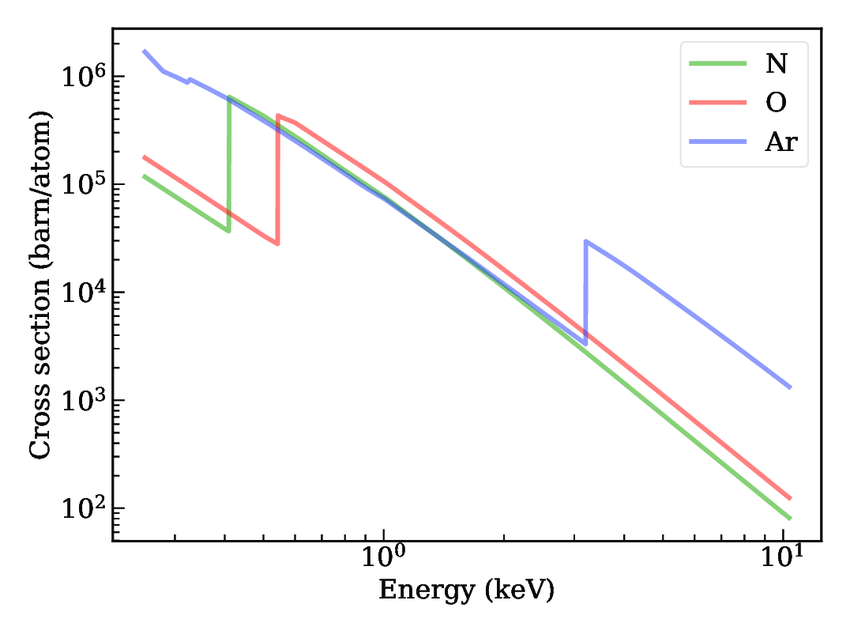
\includegraphics[width=0.75\linewidth]{Pictures/figures/photo_ion_cross_section.png}
    \caption{K-edges for various elements.}
    \label{fig:k_edges_photo_ionization}
\end{figure}

\begin{figure}
    \centering
    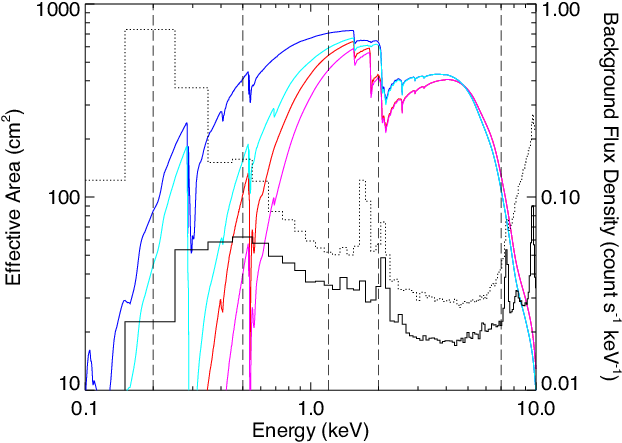
\includegraphics[width=0.75\linewidth]{Pictures//figures/chandra_effective_area.png}
    \caption{The effective area of chandra, featuring distinctive edges corresponding to the K-edges of the detector.}
    \label{fig:chandra_effective_area}
\end{figure}

For $h\nu \gg E_{\rm binding}$ but $h\nu \ll m_e c^2$, we are in a
semi--classical regime and the photoionization cross section scales as
\[
    \sigma_{\rm pi} \;\sim\; Z^5 (h\nu)^{-7/2}.
\]

\paragraph{Intuition for the scaling.}
This dependence can be understood from two complementary points of view:

\begin{itemize}
    \item \emph{$Z^5$ dependence.}  
    The hydrogenic wavefunction for an inner electron scales roughly as
    $\psi_{1s}(0) \sim Z^{3/2}$ near the nucleus. Since the transition
    probability involves the square of the matrix element, the overlap
    with the continuum grows rapidly with $Z$, leading to an overall
    scaling $\propto Z^5$ once phase--space and dipole factors are
    included. Heavier atoms therefore have much larger photoelectric
    cross sections.
    
    \item \emph{$(h\nu)^{-7/2}$ dependence.}  
    At high photon energies, the outgoing electron carries momentum
    $p \sim \sqrt{2 m_e h\nu}$ and its wavefunction oscillates rapidly.
    The overlap with the compact bound--state wavefunction is therefore
    strongly suppressed at large $p$. Quantitatively, the dipole matrix
    element falls off like $p^{-3}$ while the continuum density of
    states contributes a factor $\sim p$. Together these give a net
    $\nu^{-7/2}$ scaling of the cross section.
\end{itemize}

\begin{remark}
    \textbf{Key Points:}
    \begin{enumerate}
        \item Larger $Z$ $\;\Rightarrow\;$ much higher cross section,
              since inner--shell electrons are more tightly bound and
              concentrated near the nucleus.
        \item Larger $h\nu$ $\;\Rightarrow\;$ much lower cross section,
              since fast photoelectrons overlap poorly with the bound
              state wavefunction.
        \item This explains the characteristic behavior: large jumps at
              each absorption edge, followed by a steep decline as
              $\nu^{-7/2}$ until the next edge.
    \end{enumerate}
\end{remark}

\section{Pair-Production}

At energies higher than a few keV, the cross section for \textbf{photo-ionization drops off sharply} and we are no longer able to use the same methodologies for detectors. We therefore rely on an alternative which emerges for sufficiently high energy photons: \textbf{pair production}. There are 2 relevant mechanisms:
\begin{enumerate}
    \item \textbf{Nuclear Pair Production} $(\gamma \to e^{-} + e^{+})$ is only possible in an electro-magnetic field in order to conserve momentum and energy.
    \item \textbf{Annihilation} $(\gamma + \gamma \to e^{-} + e^{+})$.
\end{enumerate}

\subsection{Nuclear Pair Production}

Formally, $\gamma \to e^{-} + e^{+}$ cannot conserve both momentum and energy at the same time. This problem stems from the fact that the produced electrons must travel parallel to the original photon because momentum must be conserved. Working out the math, one finds that such a pair \textbf{can happen in close proximity to a nucleus}. The cross section follows the general scaling
\[
\sigma_{\rm pair} \sim \underbrace{\alpha}_{\text{fine-structure}} \sigma_T Z^2 f(\nu).
\]
\par
Another relevant feature of this emission is that we require 
\[
h \nu \ge 2 E_{\rm electron} = 2m_e c^2 \approx 1 \rm {MeV}.
\]

\subsection{Annihilation}
Famously, the inverse of the pair production process is annihilation, which produces two photons at 511 keV. We have clear evidence in our own galaxy for this process occurring.

\subsubsection{Angular Dependence}
Two photons of energies $h\nu_1$ and $h\nu_2$ colliding at angle
$\theta$ can annihilate to produce an $e^+e^-$ pair, provided there is
sufficient center--of--mass (COM) energy. The threshold condition comes
from requiring the invariant squared COM energy $s$ to exceed
$4m_e^2c^4$:
\[
    s = 2 h\nu_1 h\nu_2 (1 - \cos\theta) \;\;\geq\;\; (2m_e c^2)^2.
\]
Equivalently,
\[
    h\nu_1 h\nu_2 \;\geq\;
    \frac{(m_e c^2)^2}{1 - \cos\theta}.
\]

\paragraph{Angular dependence.}
\begin{itemize}
    \item For head--on collisions ($\theta = \pi$), the threshold is
          minimal: $h\nu_1 h\nu_2 \geq (m_e c^2)^2$.
    \item For smaller angles, the denominator decreases, raising the
          required photon energies; nearly parallel photons require
          unrealistically high energies.
\end{itemize}

\paragraph{Cross section.}
The full QED calculation gives a cross section
$\sigma_{\gamma\gamma\rightarrow e^+e^-}$ that:
\begin{enumerate}
    \item vanishes at threshold,
    \item rises rapidly just above threshold to a maximum of order
          $\sim 0.2\,\sigma_T$ (where $\sigma_T$ is the Thomson cross
          section),
    \item falls off gradually at higher energies.
\end{enumerate}
The dependence on $(1-\cos\theta)$ means that interactions are
dominated by head--on collisions.

\begin{remark}
    \textbf{Key Points:}
    \begin{enumerate}
        \item Pair production requires sufficient COM energy, expressed
              by the invariant threshold condition.
        \item The process is strongly angle dependent, favoring head--on
              photon collisions.
        \item The cross section peaks just above threshold and is always
              $\lesssim \sigma_T$.
    \end{enumerate}
\end{remark}

\section{The Combined Picture}

Having discussed the two major mechanisms for high energy photon detection, we can see that the desired bandpass of the instrument largely dictates the method of detection.

\begin{figure}[h!]
    \centering
    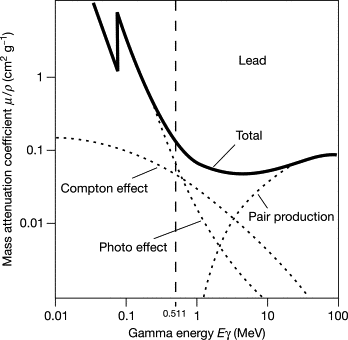
\includegraphics[width=0.75\linewidth]{Pictures//figures/gamma_cross_section.png}
    \caption{The combined cross sections for different absorption mechanisms of high energy photons.}
    \label{fig:high_energy_absorption_cross_section}
\end{figure}